% ******************************************************** %
% DOCUMENT INFORMATION                                     %
% ******************************************************** %
%                                                          %
%                                                          %
% Purpose of Document                                      %
% -------------------                                      %
% Technical Report                                         %
%                                                          %
% Institution                                              %
% -----------                                              %
% University of Applied Sciences and Arts Northwestern     %
% Switzerland, School of Engineering                       %
%                                                          %
% Degree Program                                           %
% --------------                                           %
% Electrical Engineering and Information Technology, BSc.  %
%                                                          %
% Course                                                   %
% ------                                                   %
% Project 5, Fall Semester 2016                            %
%                                                          %
% Authors                                                  %
% -------                                                  %
% Raphael Frey                                             %
% Alex Murray                                              %
%                                                          %
% Document Design and Maintenance                          %
% -------------------------------                          %
% Raphael Frey                                             %
% Based on my own work. The  template on which this report %
% was based is available at:                               %
% https://github.com/alpenwasser/longtex                   %
% -------------------------------------------------------- %

\documentclass[11pt, a4paper, oneside]{memoir}

% -------------------------------------------------------- %
% Different font and pages  sizes, layouts. Not a complete %
% list, just what I've used on occasion.                   %
% -------------------------------------------------------- %
%\documentclass[9pt,b5paper]{memoir}
%\documentclass[twocolumn,9pt,a4paper]{memoir}
%\documentclass[10pt,a5paper]{memoir} % ~60 chars per line
%\documentclass[12pt,a4paper]{memoir} % ~60 to 70 chars per line


% -------------------------------------------------------- %
% Preamble  stuff  is  kept in  the  preamble/  directory, %
% separated  out into  different files  as needed  to keep %
% things modular.                                          %
% -------------------------------------------------------- %
% -------------------------------------------------------- %
% NOTE: There   are  two   kinds  of   packages  in   this %
% document. On ond hand, there  are those which are needed %
% for this  template to function at  as intended. It might %
% still  compile without  them,  but it  will probably  no %
% longer look as it should.                                %
%                                                          %
% On the other hand, there are those which I have found to %
% be useful over the years  and tend to commonly use.  You %
% may or may  not need those.  Feel free  to disable those %
% you do not need.                                         %
%                                                          %
% By default,  I recommend leaving the  following packages %
% enabled:                                                 %
% - fontenc: for output font encoding                      %
% - inputenc: for using  non-standard characters in input, %
%   such as Umlauts or other accented characters           %
% - graphicx:  needed for  the  chapter  style (based  on  %
%   veelo)                                                 %
%                                                          %
% Feel free to  disable and enable the  rest as needed. If %
% the document no longer compiles or breaks aesthetically, %
% you will notice soon enough...                           %
% -------------------------------------------------------- %


% -------------------------------------------------------- %
% General Packages                                         %
% -------------------------------------------------------- %
\usepackage[T1]{fontenc}     % output encoding
\usepackage[utf8]{inputenc}  % input encoding
\usepackage[english]{babel}
\usepackage{lipsum}          % filler text

% -------------------------------------------------------- %
% xcolor  and kvoptions  are  loaded by  xcolor-solarized. %
% If   you  require   special   options   for  these   two %
% packages,  uncomment  these  two lines  and  pass  those %
% options. Otherwise  leave them  commented out  since the %
% packages are loaded anyway.                              %
% We load xcolor here to avoid a package option conflict   %
% -------------------------------------------------------- %
\usepackage[table]{xcolor}
%\usepackage{kvoptions}
%\usepackage[prefix=sol]{xcolor-solarized}
\usepackage{xcolor-solarized}

% -------------------------------------------------------- %
% General Packages, continued                              %
% -------------------------------------------------------- %
\usepackage{graphicx}
\usepackage{amsmath}         % for reasonable math typesetting
\usepackage{pdfpages}        % include pdf documents
\usepackage{adjustbox}       % helps w/ minipage alignmant
\usepackage{pbox}            % boxes w/ line breaks in tables
\usepackage[textsize=footnotesize, textwidth = 37mm, english, colorinlistoftodos]{todonotes}
\usepackage{calc}            % used for calculating margins and widths for A3 pages
\usepackage[separate-uncertainty=true]{siunitx}
\usepackage[light]{kpfonts}
\usepackage{counttexruns}
\usepackage[european,siunitx,cuteinductors]{circuitikz}
\usepackage{adjustbox}
\usepackage{microtype}
%\usepackage{amsfonts}        % not sure yet if we need this
%\usepackage{caption}         % captions outside float environments, overrides memoir's caption facilities
%\usepackage{subcaption} % same as the caption package, seems to override memoir's own caption configs
%\usepackage{datetime2}
\usepackage{wrapfig}
\usepackage{listings}
%\usepackage{titletoc}        % TOC per chapter

%\overfullrule=2cm


% -------------------------------------------------------- %
% Draft Watermark                                          %
%                                                          %
% Prints  a watermark  across the  page, marking  it as  a %
% draft.                                                   %
% -------------------------------------------------------- %
%\usepackage{draftwatermark}
%\SetWatermarkText{Entwurf, \today}
%\SetWatermarkScale{0.5}
%\usepackage[final]{draftwatermark} % removes watermark


% -------------------------------------------------------- %
% TIKZ and PGF                                             %
%                                                          %
% TODO: See if this  should be put in a  separate file, or %
% if  having  it  here makes  sense. Alternatively,  these %
% documents might not need to be set globally at all.      %
% -------------------------------------------------------- %
\usepackage{tikz}
\usetikzlibrary{arrows}
\usetikzlibrary{graphs}
\usetikzlibrary{spy}
\usetikzlibrary{fit}
\usetikzlibrary{backgrounds}
\usetikzlibrary{positioning}
\usetikzlibrary{shapes.misc}
\usetikzlibrary{shapes.geometric}
\usetikzlibrary{shapes.symbols}
\usetikzlibrary{decorations.pathmorphing}
\usepackage{pgfplots}
\usepackage{pgfplotstable}
%\usepgfplotslibrary{units}
\usetikzlibrary{pgfplots.units}
\pgfplotsset{compat=1.10}
\pgfplotsset{max space between ticks=80pt}
\pgfplotsset{max space between ticks=80pt}
\pgfplotsset{try min ticks=5}
\pgfplotsset{
    tick label style={font=\small},
    label style={font=\small},
    legend style={font=\footnotesize}
}
\pgfplotsset{every axis plot/.append style={%
    line width=0.5pt}}
\usepgfplotslibrary{colormaps}
\usepgfplotslibrary{external}
\tikzexternalize[prefix=cache/]

\usepackage{bytefield}


% -------------------------------------------------------- %
% Conditionals                                             %
% -------------------------------------------------------- %
% http://tex.stackexchange.com/questions/5894/latex-conditional-expression
\usepackage{etoolbox}

% -------------------------------------------------------- %
% Packages which might be used under certain circumstances %
% -------------------------------------------------------- %
%\usepackage{geometry}
%\usepackage[english]{babel}
%\usepackage{kpfonts}

% -------------------------------------------------------- %
% Set link  colors and  all that good  stuff. See hyperref %
% manual for more info and options if you wish.            %
% -------------------------------------------------------- %
\newtoggle{paper}
%\toggletrue{paper} % we're printing on paper
\togglefalse{paper} % we're making an electronic version

\iftoggle{paper}{%
    % ---------------------------------------------------- %
    % If  we're  printing on  paper,  don't  do any  fancy %
    % coloring for links and such.                         %
    % ---------------------------------------------------- %
    \usepackage[%
        bookmarksnumbered=true,
        colorlinks=true,
        linkcolor=black,
        citecolor=black,
        urlcolor=black,
        %hidelinks=false,
    ]{hyperref}
}{%
    % ---------------------------------------------------- %
    % If  we're  creating  an electronic  version  of  our %
    % document, color links as follows.                    %
    % ---------------------------------------------------- %
    \usepackage[%
        bookmarksnumbered=true,
        colorlinks=true,
        linkcolor=blue,
        citecolor=solarized-cyan,
        urlcolor=purple,
        %hidelinks=false,
    ]{hyperref}
}

% -------------------------------------------------------- %
% Input Listing Formatting                                 %
% -------------------------------------------------------- %
\lstdefinestyle{txt}{
    aboveskip           = 3mm,
    belowskip           = 3mm,
    showstringspaces    = false,
    columns             = flexible,
    keepspaces          = true,
    basicstyle          = {\scriptsize\ttfamily},
    numbers             = left,
    numberstyle         = \tiny\color{gray},
    breaklines          = true,
    breakatwhitespace   = true,
    tabsize             = 3
}

% -------------------------------------------------------- %
% This file contains various options for the memoir class  %
% itself.                                                  %
% -------------------------------------------------------- %


% -------------------------------------------------------- %
% Rename Appendices to whatever we want.                   %
% See p78 of memman.pdf                                    %
% -------------------------------------------------------- %
%\def\appendixpagename{\sffamily\HUGE Anh\"ange}
%\def\appendixtocname{Anh\"ange}

% -------------------------------------------------------- %
% Choose a page layout                                     %
% -------------------------------------------------------- %
%                                                          %
% The  layout  is based  on isopage,  with  the  following %
% changes:                                                 %
% - The spine margin is 30 mm. This is so that binding the %
% document with  a ringbinder does  not come too  close to %
% the text.                                                %
% - The edge  margin is  1.5 times the spine  margin, i.e. %
% 45 mm.                                                   %
% - The top margin is 1/9  of the paper height, same as in %
% \isopage                                                 %
% - The bottom margin is decreased from isopage's value to %
% 1.5 times the top margin, i.e. about 50 mm.              %
% -------------------------------------------------------- %

%    +----------^--------------------+
%    |          | 33mm               |
%    |     +----v------------+       |
%    |30mm |                 | 45mm  |
%    |<--->|                 |<----->|
%    |     |                 |       |
%    |     |                 |       |
%    |     |                 |       |
%    |     |                 |       |
%    |     |                 |       |
%    |     |                 |       |
%    |     |                 |       |
%    |     |                 |       |
%    |     |                 |       |
%    |     |                 |       |
%    |     |                 |       |
%    |     |                 |       |
%    |     +----^------------+       |
%    |          | 49.5mm             |
%    |          |                    |
%    +----------v--------------------+
\isopage%
\setlrmarginsandblock{0.142857111\paperwidth}{0.190476190\paperwidth}{*}
\setulmarginsandblock{0.111111111\paperheight}{*}{1.5}%
\checkandfixthelayout%


% -------------------------------------------------------- %
% Choose a chapter style                                   %
% We're  going  with  veelo, but  removing  the  "Chapter" %
% designation in front of the chapter number.              %
% -------------------------------------------------------- %
% -------------------------------------------------------- %
% This  chapterstyle is  baesd on  veelo, but  removes the %
% "Chapter" designation in front of the chapter number.    %
% -------------------------------------------------------- %
%
% TODO: Check if this is allowed by the  LPPL, under which
% 'memoir.cls' is distributed, which contains the original
% code for the veelo chapter style.
%
% http://www.latex-project.org/lppl.txt
%
% If this is not permitted, implement alternative via this:
% http://tex.stackexchange.com/questions/51527/chapter-heading-with-the-word-chapter-replaced-by-chapter-name

\makeatletter
\makechapterstyle{fhnw}{%
    \setlength{\afterchapskip}{40pt}
    \renewcommand*{\chapterheadstart}{\vspace*{40pt}}
    \renewcommand*{\afterchapternum}{\par\nobreak\vskip 25pt}
    \renewcommand*{\chapnamefont}{\sffamily\LARGE\flushright}
    \renewcommand*{\chapnumfont}{\sffamily\HUGE}
    \renewcommand*{\chaptitlefont}{\sffamily\HUGE\bfseries\flushright}
    \renewcommand*{\printchaptername}{%
        \chapnamefont\MakeTextUppercase{}}
    \renewcommand*{\chapternamenum}{}
    \setlength{\beforechapskip}{18mm}%  \numberheight
    \setlength{\midchapskip}{\paperwidth}% \barlength
    \addtolength{\midchapskip}{-\textwidth}
    \addtolength{\midchapskip}{-\spinemargin}
    \renewcommand*{\printchapternum}{%
        \makebox[0pt][l]{%
            \hspace{.8em}%
            \resizebox{!}{\beforechapskip}{\chapnumfont \thechapter}%
            \hspace{.8em}%
            \rule{\midchapskip}{\beforechapskip}%
        }%
    }%
   \makeoddfoot{plain}{}{}{\thepage}%
}
\makeatother

\chapterstyle{fhnw} % requires graphicx package

\setsecheadstyle{\Large\bfseries\sffamily}
\setsubsecheadstyle{\large\bfseries\sffamily}
\setsubsubsecheadstyle{\bfseries\sffamily}

% -------------------------------------------------------- %
% Pagestyle (Headers, Footers)                             %
% -------------------------------------------------------- %
\pagestyle{headings}

% -------------------------------------------------------- %
% Cross Referencing Stuff                                  %
% -------------------------------------------------------- %

% Apparently these are not automatically translated into
% German by babel:
\def\figurerefname{Abbildung}
\def\tablerefname{Tabelle}
\def\pagerefname{Seite}

% -------------------------------------------------------- %
% Caption Configurations                                   %
% -------------------------------------------------------- %
\captionnamefont{\bfseries\small}
\captiontitlefont{\small}
\captiondelim{: }

% Captions for use outside of floats
\newfixedcaption{\figcaption}{figure}
\newfixedcaption{\tabcaption}{table}

% -------------------------------------------------------- %
% Define  what  sort  of  sectional  divisions  should  be %
% numbered.  See also "Document Divisions -- Numbering" in %
% the memoir manual.                                       %
%                                                          %
%            Division            |  Level                  %
%          ----------------------+---------                %
%            \book               |  -2                     %
%            \part               |  -1                     %
%            \chapter            |   0                     %
%            \section            |   1                     %
%            \subsection         |   2                     %
%            \subsubsection      |   3                     %
%            \paragraph          |   4                     %
%            \subparagraph       |   5                     %
%                                                          %
% \setsecnumdepth{<division>} sets  division numberings so %
% that <division>  and above will be  numbered.  When used %
% in  the preamble  (such as  here), \setsecnumdepth  also %
% calls \maxsecnumdepth, which is the numbering level used %
% in the \mainmatter part of the document. \setsecnumdepth %
% can be used anywhere  in the mainmatter to (temporarily) %
% change the numbering level.                              %
%                                                          %
% This template  uses chapters, sections,  subsections and %
% subsubsections  by default,  so  we  will set  numbering %
% level to subsubsection per default. Adjust as needed. We %
% will set this to subsubsection per default.              %
% -------------------------------------------------------- %
\setsecnumdepth{subsubsection}
\maxsecnumdepth{subsubsection}
\settocdepth{subsubsection}
\maxtocdepth{subsubsection}

\def\code#1{\texttt{#1}}
\def\quelleVA{\emph{Quelle:} Versuchsanleitung}
\def\anweisung{\emph{Anmerkung f\"ur Autoren: }}
\def\Raspi{Raspberry Pi}
\def\ISC{I\textsuperscript{2}C}


\definecolor{darkred}{rgb}{0.7,0,0}
\definecolor{darkblue}{rgb}{0.6,0.6,1}
\definecolor{darkgray}{gray}{0.4}
% checkmark
\newcommand{\checkmark}{\tikz\fill[fill=black!30!green,scale=0.4](0,.35) -- (.25,0) -- (1,.7) -- (.25,.15) -- cycle;}
% partially fulfilled
\newcommand{\partially}{\tikz\fill[fill=darkblue,scale=0.4](.5,0) -- (.55,.28) -- (.8,.33) -- (.55,.38) -- (.55,.62) -- (.8,.67) -- (.55,.72) -- (.5,1) -- (.45,.72) -- (.2,.67) -- (.45,.62) -- (.45,.38) -- (.2,.33) -- (.45,.28) -- cycle;}
% no indication
\newcommand{\noi}{\textcolor{darkgray}{\small\textsf{---}}}
% not present
\newcommand{\np}{\tikz\fill[fill=darkred,scale=0.4](0,0) -- (.5,.4) -- (1,0) -- (.6,.5) -- (1,1) -- (.5,.6) -- (0,1) -- (.4,.5) -- cycle;}
%\newcommand{\nv}{\textcolor{darkred}{$×$}}

\newcommand{\Sensor}{Sensor}
\newcommand{\Master}{Master-Ger\"at}

\newcommand{\myfancybreaksymbol}{\Diamond}
\newcommand{\myfancybreak}{\fancybreak{$\myfancybreaksymbol\quad\myfancybreaksymbol\quad\myfancybreaksymbol$}}

\newlength{\parindentbak}

\newcommand{\colorbitbox}[4]{%
    \rlap{\bitbox{#3}{\color{#1}\rule{\width}{\height}}}%
    \bitbox{#3}{\sffamily\textcolor{#2}{#4}}}

\newenvironment{conditions}
  {\noindent Wobei: \par\vspace{\abovedisplayskip}\noindent\begin{tabular}{>{$}l<{$} @{${}:{}$} l}}
  {\end{tabular}\par\vspace{\belowdisplayskip}}

% -------------------------------------------------------- %
% Provides  a   new  environment  a3pages   for  inserting %
% landscape a3pages at arbitrary points in your document.  %
%                                                          %
% NOTE: This environment needs to be enclosed in braces to %
% work  correctly.  Unfortunately,  I  haven't managed  to %
% integrate  those into  the commands  directly yet  (they %
% obviously mess up the bracing of the command itself).    %
%                                                          %
% EXAMPLE:                                                 %
%                                                          %
% {\begin{a3pages}                                         %
%     your content                                         %
%     goes here                                            %
%     and will be put on                                   %
%     landscape A3 pages                                   %
% \end{a3pages}}                                           %
%                                                          %
% Note the  opening brace  before \begin{a3pages}  and the %
% additional closing brace after \end{a3pages}             %
% -------------------------------------------------------- %
% See also:
% http://tex.stackexchange.com/questions/16942/difference-between-textwidth-linewidth-and-hsize

\newenvironment{a3pages}
    {%
        \clearpage
        \setlength{\pdfpagewidth}{2\pdfpagewidth}
        \setlength{\hsize}{\pdfpagewidth-\spinemargin-\foremargin} % for text paragraphs
        \setlength{\textwidth}{\hsize}                             % headers, footers
        \setlength{\stockwidth}{2\stockwidth}
        \setlength{\paperwidth}{2\paperwidth}
        \checkandfixthelayout%
    }
    {%
        \clearpage
    }



% -------------------------------------------------------- %
% If only some files are to  be included in the file for a %
% compilation run, specify those files here.               %
% -------------------------------------------------------- %
%\includeonly{%
%    frontmatter/info,
%    frontmatter/abstract,
%    mainmatter/einleitung,
%    mainmatter/uberblick,
%    mainmatter/models,
%    mainmatter/simu,
%    mainmatter/hardware,
%    mainmatter/hardware-sensor,
%    mainmatter/hardware-master,
%    mainmatter/software,
%    mainmatter/firmware-sensor,
%    mainmatter/software-master,
%    mainmatter/validierung,
%    mainmatter/userguide,
%    mainmatter/fazit,
%    appendices/commercial-modules,
%    appendices/ltspice,
%    appendices/schema,
%    appendices/validierung,
%    appendices/costs,
%    appendices/datentrager,
%}

% ******************************************************** %
\begin{document}
% ******************************************************** %
%\fontfamily{pbk}\selectfont

% -------------------------------------------------------- %
% NOTE: The titlepage will also leave one empty page after %
% itself, so that it doesn't  get its backside printed for %
% double-sided  printing. If  document  has  been  set  to %
% single-sided  printing,  no  empty verso  page  will  be %
% added.                                                   %
% -------------------------------------------------------- %
\begin{titlingpage}

    %\bfseries

    % ---------------------------------------------------- %
    % Main Info on Contents                                %
    % ---------------------------------------------------- %
    \newcommand{\infotable}{%
        \begin{tabular}{r|l}
            \textsc{\textbf{Degree Program}}
            & Electrical Engineering and Information Technology \\
            [4mm]

            \textsc{\textbf{Course}}
            & Project 5 \\
            [4mm]

            \textsc{\textbf{Advisors}}
            & Alex Huber, Hanspeter Schmid \\
            [4mm]

            \textsc{\textbf{Authors}}
            & Raphael Frey, Alex Murray \\
            [4mm]

            \textsc{\textbf{Date}}
            & \today \\
            [4mm]

            \textsc{\textbf{Version}}
            & 0.2 \\
        \end{tabular}%
    }%


    % ---------------------------------------------------- %
    % Place the Background Picture and Info Table          %
    % ---------------------------------------------------- %
    \hspace{-2.54mm}
    \newlength{\logoX}
    \setlength{\logoX}{5mm}
    \newlength{\logoY}
    \setlength{\logoY}{5mm}
    \begin{tikzpicture}[remember picture, overlay]
        % ------------------------------------------------ %
        % Background Picture                               %
        % ------------------------------------------------ %
        %\node[inner sep=0pt] at (current page.center) {%
        %    \includegraphics[width=\paperwidth,height=\paperheight]{images/titlepage/titlepic.jpg}%
        %};
        %\node[
        %    fill=white,
        %    fill opacity=0.5,
        %    inner sep=0pt,
        %    anchor=west
        %] at (-38.5mm,-105mm) {%
        %    \input{images/python/title.pgf}%
        %};

        % ------------------------------------------------ %
        % Info Table                                       %
        % ------------------------------------------------ %
        \node[%
            %fill=black,
            %fill opacity=0.8,
            %rounded corners=10mm,
            %outer sep=0pt,
            inner sep=2em,
            yshift=9em,
            anchor = south,
        ] at (current page.south) {\textcolor{black}{\infotable}};

        % ------------------------------------------------ %
        % FHNW Logo                                        %
        % ------------------------------------------------ %
        \node[anchor=north west,xshift=\logoX,yshift=-\logoY,outer sep=0pt,inner sep=0pt] at (current page.north west) {%
            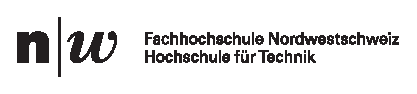
\includegraphics[height=12mm]{images/titlepage/fhnw.eps}%
        };
    \end{tikzpicture}



    % ---------------------------------------------------- %
    % The Text can  be set rather low in  the page without %
    % adjusting the top lengths.                           %
    % Backing up  and reseting these lengths  seems not to %
    % be necessary;  it appears  they are restored  at the %
    % end of the titlingpage environment.                  %
    % ---------------------------------------------------- %
    \setlength{\headsep}{0pt}
    \setlength{\headheight}{0pt}
    \setlength{\uppermargin}{4em}
    \checkandfixthelayout


    % ---------------------------------------------------- %
    % By   default,  centering   inside  the   titlingpage %
    % environment  will   center  with  respects   to  the %
    % typeblock. When  the  typeblock  is  centered,  this %
    % leads to  centered text  with respect to  the entire %
    % title  page. However,  When  the  typeblock  is  not %
    % centered, some adjustment is needed.                 %
    % See memman Chapter "Titles" for more information.    %
    % ---------------------------------------------------- %
    \calccentering{\unitlength}
    \begin{adjustwidth*}{\unitlength}{-\unitlength}


    % ---------------------------------------------------- %
    % Work some  magic to  automatically adjust  the hrule %
    % lengths to the length of the book title.             %
    %                                                      %
    % NOTE: The  font  size setting  needs  to  be in  the %
    % \mytitle  command, otherwise  \settolength will  not %
    % take it  into account  and will only  calculate with %
    % the default font size.                               %
    %                                                      %
    % NOTE  2: This mechanism  breaks if  the title  spans %
    % across multiple  lines. You're on  your own  in that %
    % case.                                                %
    % ---------------------------------------------------- %
    %\newcommand{\mytitle}{{\textbf{\fontsize{25mm}{1em}\selectfont Project Powerline}}} % default font
    \vspace*{7em}
    \newcommand{\mytitle}{{\textbf{\fontsize{12mm}{1em}\selectfont Sensor Chip}}}
    \newlength{\titlelength}            % Length of title text
    \settowidth{\titlelength}{\mytitle}
    \newcommand{\titlerulefactor}{1.2}  % Length of title rules, as a factor

    % ---------------------------------------------------- %
    % Set the title color                                  %
    % ---------------------------------------------------- %
    \newcommand{\titlecolor}{black}

    % ---------------------------------------------------- %
    % Put the title onto the page                          %
    % ---------------------------------------------------- %
    \textcolor{\titlecolor}{%
        \centering
        \rule{\titlerulefactor\titlelength}{1pt} \\
        \vspace*{4mm}
        \mytitle\\
        %\vspace*{5mm}
        \rule{\titlerulefactor\titlelength}{1pt} \\
        \vspace*{6mm}
        \fontsize{8mm}{1em}\selectfont Technical Report \\
    }


    % ---------------------------------------------------- %
    % This is the end of the centering magic.              %
    % ---------------------------------------------------- %
    \end{adjustwidth*}


    % ---------------------------------------------------- %
    % Make  sure  this  is   not  put  into  \frontmatter, %
    % otherwise it will get a \frontmatter folio.          %
    % \cleardoblepage  is not  actually necessary  because %
    % it  is  automatically   called  by  the  titlingpage %
    % environment.                                         %
    % ---------------------------------------------------- %
    %\cleardoublepage

    %\setlength{\headsep}{\originallength}
    %\checkandfixthelayout
\end{titlingpage}


% -------------------------------------------------------- %
% See  the  memoir  documentation  for  what  specifically %
% frontmatter does. Among  other things, page  numbers are %
% set to roman numerals and chapter numbers are removed.   %
% -------------------------------------------------------- %
\frontmatter

% -------------------------------------------------------- %
% Comment out what's not needed, obviously.                %
% -------------------------------------------------------- %
%\begin{centering}
\vspace*{30mm}
\begin{tiny}
    \begin{tabular}{lll}
        Content & \copyright~2016 & Raphael Frey \\
                &                 & Alex Murray  \\
                &                 &              \\
        Design  & \copyright~2016 & Raphael Frey \\
    \end{tabular}


    % ---------------------------------------------------- %
    % Having  this  in  a  tabular  is  a  bit  ugly,  but %
    % it  ensures alignment  and  limited paragraph  width %
    % without much effort.                                 %
    % ---------------------------------------------------- %
    \vspace{1em}
    \begin{tabular}{p{.9\textwidth}}
        \noindent Created in fall semester 2016 at the FHNW School for Engineering.\\

        \\
        \iftoggle{paper}{%
            This is the print version  of this document. An electronic version
            with colored and clickable yperlinks  is available upon request at
            \code{rmfrey@runbox.com}.
        }{%
            This is the electronic version of this document. Hyperlinks are colored
            and clickable. For a version with non-colored hyperlinks, please contact
            \href{mailto:rmfrey@runbox.com}{\code{rmfrey@runbox.com}}.
            % internet links: blau
            % externe links: magenta
        }
        \\

        \\
        This document has been compiled \thecounttexruns~times so far.\\
    \end{tabular}
    \vspace{1em}

    \begin{tabular}{>{\ttfamily}lrl}
        Version 0.1 & 10.10.2016 & Creation \\
    \end{tabular}

    \vspace{1em}
    %\begin{tabular}{l @{${}:{}$} l}
    %    Source title image & \cite{ref:titlepage:pvanlage} \\
    %    Source Logo FHNW & \cite{ref:fhnwlogo}           \\
    %\end{tabular}
\end{tiny}
%\\
%\footnotesize{\checkmark~\np~\noi~\partially} \\
%\\
%\large{\checkmark~\np~\noi~\partially} \\
%\\
%\checkmark~\np~\noi~\partially
%\end{centering}

%% ---------------------------------------------------------------------------- %
\chapter*{Abstract}
\label{ch:abstract}
% ---------------------------------------------------------------------------- %

As an ongoing  project at the Institute of Microelectronics,  a \sdm~ has been
in development over the past few years. This project's objective was to develop
a comprehensive  test and  data processing suite  to efficiently  and reliably
assess the performance  of various verions of these chips. In  a second stage,
the results of these measurements are to be used to further improve the \sdm's
design.

A  test  bench  has been  developed  which  allows  measurement of ten  chips  in
a  few  days  in  various configurations. The  measurement  process  has  been
largely automated  with scripts, requiring little  manual intervention. In our
project, this  has resulted  in roughly \num{4000}  measurements, representing
about \num{500000000} measurement points  and requiring approximately \num{12}
gigabytes  of storage  space. The setup  has  been documented  so that  future
groups can rebuild it and reproduce our results.

TODO: Stuff from Alex.

%\include{frontmatter/dedication}
%\include{frontmatter/declaration}
%\include{frontmatter/acknowledgements}


% -------------------------------------------------------- %
% The starred versions do not make an entry for themselves %
% in the ToC, the unstarred versions do.                   %
% -------------------------------------------------------- %
{%
\enlargethispage{4em}
\tableofcontents*
}
%\newpage\listoffigures
%\newpage\listoftables


% -------------------------------------------------------- %
% Set page numbers to  arabic numerals, reset page counter %
% to 1, display  chapter numbers. See memoir documentation %
% for more information.                                    %
% -------------------------------------------------------- %
\mainmatter


% -------------------------------------------------------- %
% It is  advisable to use actually  meaningful chapter and %
% section names instead of generically numbered ones as in %
% this  example structure. That  way, their  place in  the %
% document is not directly tied to their file name, and it %
% is  possible to  restructure the  document (e.g.  move a %
% section  from one  chapter  to another,  or reorder  the %
% chapters)  without  needing  to adjust  file  names  and %
% similar shenanigans.                                     %
% -------------------------------------------------------- %
%\include{mainmatter/einleitung}


% -------------------------------------------------------- %
% Appendices are  usually numbered  and therefore  part of %
% the mainmatter, not the backmatter.                      %
% The advice about meaningful chapter names applies to the %
% appendices as well, see above.                           %
% -------------------------------------------------------- %
\appendixpage
\appendix
%\include{appendices/ltspice}
%\include{appendices/costs}
%\include{appendices/datentrager}


% -------------------------------------------------------- %
% Page  numbering continues,  but chapter  numbers are  no %
% longer  displayed. See  memoir  documentation  for  more %
% information.                                             %
% -------------------------------------------------------- %
\backmatter

% -------------------------------------------------------- %
% Bibliography: We  are using  the  IEEEtran package  from %
% Michael Shell                                            %
%                                                          %
% There  are  a  few  different  styles  in  the  IEEEtran %
% package.   We are  going to  use  one of  two of  those, %
% either in the sorted or unsorted variety.                %
%                                                          %
% The sorted  version sorts  bibliographic entries  in the %
% bibliography alphabetically, while  the unsorted version %
% lists bibliographic  entries in the order  in which they %
% were cited (first occurrence).                           %
% -------------------------------------------------------- %
%\bibliographystyle{bibliography/IEEEtranS} % sorted
\raggedright
\bibliographystyle{bibliography/IEEEtran} % unsorted
\bibliography{bibliography/references}
\end{document}
